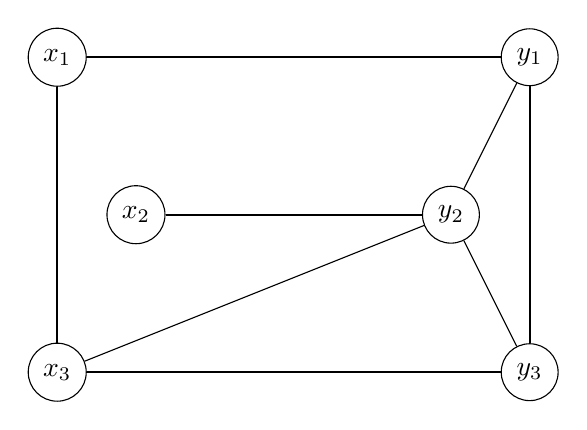
\begin{tikzpicture}[yscale=-1,scale=2]
\node[draw=black,circle] (Nx1) at (0,0) {$x_1$};
\node[draw=black,circle] (Nx3) at (0,2) {$x_3$};
\node[draw=black,circle] (Ny1) at (3,0) {$y_1$};
\node[draw=black,circle] (Ny3) at (3,2) {$y_3$};
\node[draw=black,circle] (Nx2) at (0.5,1) {$x_2$};
\node[draw=black,circle] (Ny2) at (2.5,1) {$y_2$};
\draw[thick] (Nx1) -- (Ny1);
\draw[thick] (Nx3) -- (Ny3);
\draw[thick] (Nx1) -- (Nx3);
\draw[thick] (Ny1) -- (Ny3);
\draw[thick] (Nx2) -- (Ny2);
\draw (Ny1) -- (Ny2);
\draw (Ny2) -- (Ny3);
\draw (Nx3) -- (Ny2);
\end{tikzpicture}